\documentclass[12pt]{article}
\usepackage[margin=1in]{geometry}
\usepackage[utf8]{inputenc}
\usepackage[LGR,T1]{fontenc}
\usepackage[greek,english]{babel}
\usepackage{alphabeta}
\usepackage{listings}
\usepackage{xcolor}
\usepackage{booktabs}
\usepackage{graphicx}
\usepackage{amsmath}
\usepackage{float}
\usepackage[unicode]{hyperref}
\usepackage{tikz}
\usetikzlibrary{arrows.meta, positioning, fit}
\addto\captionsenglish{\renewcommand{\partname}{Μέρος}}

\lstset{
    language=Python,
    basicstyle=\ttfamily\small,
    keywordstyle=\color{blue},
    stringstyle=\color{orange},
    commentstyle=\color{gray},
    frame=single,
    breaklines=true,
}

\title{SLP Lab 2: Sentiment Analysis Report\\[0.3em]\large Προπαρασκευή \& Κυρίως Εργαστήριο}
\author{}
\date{}

\begin{document}
\maketitle

\part{Προπαρασκευή}

%-----------------------------------------------------------------------
\section{Φόρτωση και Προεπεξεργασία Δεδομένων}

\subsection{Ζητούμενο 1: Κωδικοποίηση Επισημειώσεων}

Οι επισημειώσεις (labels) κωδικοποιούνται σε ακέραιους μέσω του
\texttt{LabelEncoder} του scikit-learn, ο οποίος ταξινομεί αλφαβητικά
τις μοναδικές ετικέτες και τους αποδίδει μηδενο-βασισμένους δείκτες.
Η αντιστοίχιση εφαρμόζεται ταυτόχρονα στο training και test set, ώστε
να είναι συνεπής.

\begin{lstlisting}
DEBUG = True   # global flag -- set False to silence all debug prints

# EX1 -- label encoding
le = LabelEncoder()
le.fit(y_train)
y_train = le.transform(y_train)
y_test  = le.transform(y_test)

if DEBUG:
    print("Classes:", le.classes_)
    print("First 10 raw labels:", list(y_train_raw[:10]))
    print("First 10 encoded:   ", y_train[:10])
\end{lstlisting}

Παράδειγμα εξόδου για \textbf{MR}:

\begin{lstlisting}[language={}]
[MR] EX1 -- Label encoding
  Classes:             ['negative' 'positive']
  First 10 raw labels: ['positive', 'positive', 'positive', 'positive',
                        'positive', 'positive', 'positive', 'positive',
                        'positive', 'positive']
  First 10 encoded:    [1 1 1 1 1 1 1 1 1 1]
\end{lstlisting}

Για το \textbf{Semeval2017A} (τρίκλαση):
\texttt{negative}~$\to 0$, \texttt{neutral}~$\to 1$, \texttt{positive}~$\to 2$.

\subsection{Ζητούμενο 2: Λεκτική Ανάλυση (Tokenization)}

Κάθε πρόταση μετατρέπεται σε ακολουθία tokens μέσω του
\texttt{TweetTokenizer} της βιβλιοθήκης NLTK, ο οποίος χειρίζεται
σωστά στοιχεία κοινωνικών δικτύων (hashtags, mentions, emoticons).
Κάθε token αντιστοιχίζεται στον ακέραιο δείκτη του στο λεξιλόγιο
των embeddings· οι λέξεις εκτός λεξιλογίου (OOV) αντιστοιχίζονται
στο token \texttt{$<$unk$>$}.

\subsection{Ζητούμενο 3: \texttt{\_\_getitem\_\_}}

Η μέθοδος \texttt{\_\_getitem\_\_} επιστρέφει τρία στοιχεία:
\begin{enumerate}
    \item την κωδικοποιημένη ακολουθία δεικτών λέξεων (με zero-padding ή truncation στο \texttt{max\_length}~$=40$),
    \item την ακέραια ετικέτα κλάσης,
    \item το πραγματικό μήκος της πρότασης (εξαιρώντας τα μηδενικά padding).
\end{enumerate}
Το \texttt{max\_length} επιλέχθηκε ώστε να καλύπτει την πλειοψηφία
των μηκών πρότασης στα training sets.

%-----------------------------------------------------------------------
\section{Μοντέλο}

\subsection{Ζητούμενο 4: Embedding Layer}

Το embedding layer αρχικοποιείται από τα προ-εκπαιδευμένα word
embeddings και παγώνεται κατά την εκπαίδευση.

\textbf{Γιατί αρχικοποιούμε από προ-εκπαιδευμένα embeddings;}
Τα embeddings (π.χ.\ GloVe) εκπαιδεύονται σε δισεκατομμύρια tokens
και κωδικοποιούν πλούσιες σημασιολογικές σχέσεις μεταξύ λέξεων.
Αποτελούν ένα ποιοτικό σημείο εκκίνησης που θα ήταν αδύνατο να
μάθουμε από τα μικρά sentiment datasets.

\textbf{Γιατί παγώνουμε τα βάρη;}
Το embedding layer περιέχει πολύ περισσότερες παραμέτρους από τον
υπόλοιπο ταξινομητή. Η ενημέρωσή τους σε ένα μικρό dataset θα
αλλοίωνε τη δομή του χώρου embeddings --- ουσιαστικά θα οδηγούσε
σε overfitting.

\subsection{Ζητούμενο 5: Output Layers}

Πριν το τελικό γραμμικό layer τοποθετείται ένας μη-γραμμικός
μετασχηματισμός (ReLU).

\textbf{Γιατί απαιτείται μη-γραμμικότητα;}
Η σύνθεση γραμμικών μετασχηματισμών παραμένει γραμμική:
$\mathbf{y} = W_2(W_1\mathbf{x}) = (W_2 W_1)\mathbf{x}$.
Ανεξαρτήτως πλήθους layers, η κλάση αναπαραστάσιμων συναρτήσεων
$\mathcal{H}$ παραμένει η ίδια --- αυτή των αφφινικών απεικονίσεων.
Η εισαγωγή μιας μη-γραμμικής ενεργοποίησης (π.χ.\ ReLU) σπάει
αυτή την ισοδυναμία, επιτρέποντας μη-γραμμικά όρια απόφασης και
αυξάνοντας την εκφραστική δύναμη του μοντέλου.

\subsection{Ζητούμενο 6: Forward Pass}

Το forward pass εκτελεί τα εξής βήματα:
\begin{align}
    E &= \text{embed}(x) && \text{(}B \times T \times d\text{)} \label{eq:embed}\\
    u &= \frac{1}{N}\sum_{i=1}^{N} e_i && \text{μέσος όρος embeddings} \label{eq:mean}\\
    r &= \text{ReLU}(Wu + b) && \text{μη-γραμμικός μετασχηματισμός} \label{eq:relu}\\
    \hat{y} &= W_o r + b_o && \text{προβολή στις κλάσεις} \label{eq:proj}
\end{align}

\textbf{Διαισθητική ερμηνεία του κέντρου βάρους.}
Αν κάθε διάσταση του embedding χώρου αντιστοιχεί σε μια αφηρημένη
σημασιολογική ιδιότητα, τότε το κέντρο βάρους εκφράζει το ``μέσο
σημασιολογικό προφίλ'' της πρότασης. Για παράδειγμα, αν μια
διάσταση συσχετίζεται με \emph{ένταση συναισθήματος}, η πρόταση
``a thrilling, breathtaking masterpiece'' θα έχει υψηλή τιμή
σε αυτή τη διάσταση.

\textbf{Αδυναμίες:}
\begin{itemize}
    \item \textbf{Απώλεια σειράς λέξεων.} Το κέντρο βάρους είναι
    αναλλοίωτο σε αναδιατάξεις: ``not expensive'' και ``expensive not''
    δίνουν ίδια αναπαράσταση. Η άρνηση (negation) χάνεται.
    \item \textbf{Αγνόηση πλαισίου.} Κάθε λέξη λαμβάνει σταθερό
    embedding ανεξάρτητα από τα συμφραζόμενα --- πολυσημία όπως
    ``bank'' (ποτάμι vs.\ τράπεζα) δεν αποσαφηνίζεται.
\end{itemize}

%-----------------------------------------------------------------------
\section{Εκπαίδευση}

\subsection{Ζητούμενο 7: DataLoaders}

\textbf{Μέγεθος mini-batch.}
Η διακύμανση του σφάλματος ανά batch είναι
$\mathrm{Var}(L_B) = \sigma_\ell^2 / |B|$,
όπου $\sigma_\ell^2$ η διακύμανση ανά δείγμα.
Μικρά batches δίνουν θορυβώδεις ενημερώσεις
(ρυθμιστικό αποτέλεσμα, λιγότερο overfitting),
ενώ μεγάλα batches σταθερή σύγκλιση αλλά τάση
συγκέντρωσης σε ``αιχμηρά'' ελάχιστα.

\textbf{Γιατί ανακατεύουμε (shuffle);}
Χωρίς ανακάτεμα, τα ίδια δείγματα σχηματίζουν πάντα τα ίδια batches
και εμφανίζονται στην ίδια σειρά, εισάγοντας σειριακή μεροληψία.
Η ανακατανομή εξασφαλίζει πιο αντιπροσωπευτικές εκτιμήσεις gradient
ανά εποχή.

\subsection{Ζητούμενο 8: Συνάρτηση Σφάλματος, Παράμετροι, Optimizer}

\begin{itemize}
    \item \textbf{Loss:} Για δυαδική κατηγοριοποίηση (MR) χρησιμοποιούμε
    \texttt{BCEWithLogitsLoss} (ένα logit, sigmoid + BCE). Για τρεις
    κλάσεις (Semeval2017A) χρησιμοποιούμε \texttt{CrossEntropyLoss}
    (softmax + NLL).
    \item \textbf{Παράμετροι:} Μόνο οι παράμετροι με
    \texttt{requires\_grad=True} περνούν στον optimizer ---
    τα παγωμένα embeddings εξαιρούνται.
    \item \textbf{Optimizer:} Adam (adaptive learning rate ανά
    παράμετρο μέσω running moments).
\end{itemize}

\subsection{Ζητούμενο 9: Βρόχοι Εκπαίδευσης και Αξιολόγησης}

Η \texttt{train\_dataset} εκτελεί forward pass, υπολογίζει το loss,
κάνει backpropagation και ενημερώνει τα βάρη (SGD step).
Η \texttt{eval\_dataset} αξιολογεί χωρίς gradient, υπολογίζοντας
τις προβλέψεις: threshold στο μηδέν (sign of logit) για BCEWithLogitsLoss
ή $\arg\max$ για CrossEntropyLoss.

%-----------------------------------------------------------------------
\section{Αξιολόγηση}

\subsection{Ζητούμενο 10: Μετρικές και Καμπύλες Εκπαίδευσης}

\begin{figure}[H]
\centering
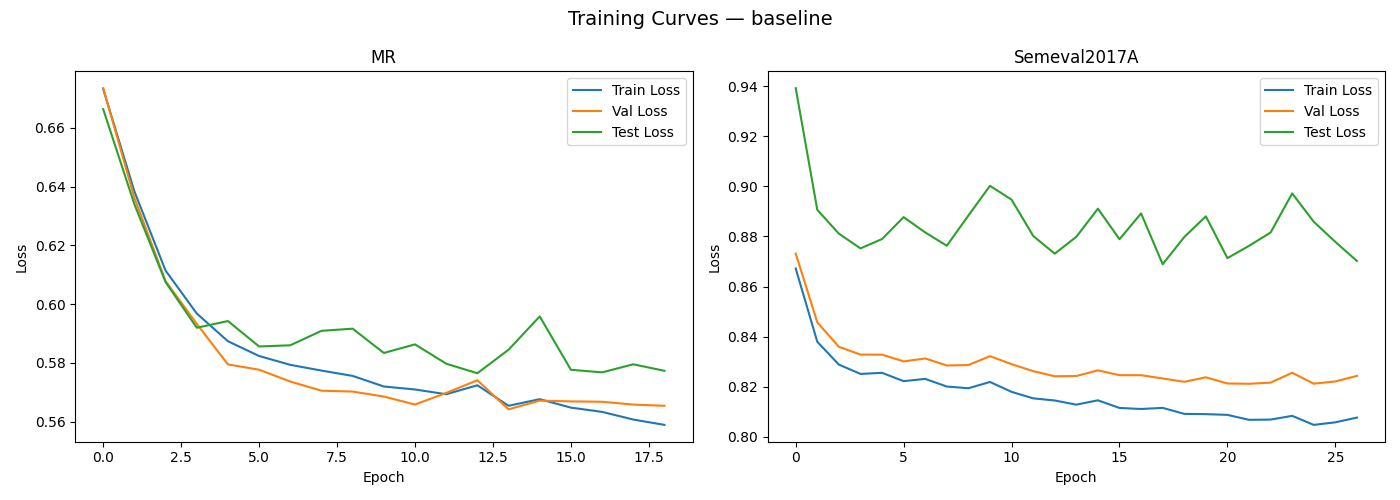
\includegraphics[width=\textwidth]{results/loss_baseline.png}
\caption{Καμπύλες εκπαίδευσης του Baseline DNN (mean pooling) στο MR (αριστερά) και Semeval2017A (δεξιά).}
\end{figure}

\lstinputlisting[language={}, firstline=21, lastline=32]{results/baseline_results.txt}

Το μοντέλο επιτυγχάνει $\sim$70\% F1 στο MR και $\sim$53\% στο Semeval2017A.
Η χαμηλότερη επίδοση στο Semeval εξηγείται τόσο από την τρίτη (neutral)
κλάση όσο και από τη θορυβώδη φύση των tweets.

\subsection{Ζητούμενο 11: Κατηγοριοποίηση με LLM (ChatGPT)}

Δοκιμάσαμε το ChatGPT (GPT-4) σε zero-shot κατηγοριοποίηση
συναισθήματος, χρησιμοποιώντας κατάλληλα prompts.

\subsubsection*{MR Dataset}

Επιλέχθηκαν 40 κριτικές ταινιών (20 θετικές, 20 αρνητικές).
Στο prompt ανατέθηκε ο ρόλος ``expert movie critic and sentiment
analyzer'' και ζητήθηκε ταξινόμηση σε Positive/Negative.

\textbf{Αποτέλεσμα: Accuracy $= 1.0$ (40/40 σωστά).}

Σε δεύτερο prompt ζητήθηκε ανάλυση 6 αντιπροσωπευτικών
παραδειγμάτων (3 εύκολα, 3 δύσκολα):
\begin{itemize}
    \item \textit{Εύκολα:} Λέξεις-κλειδιά όπως ``masterpiece'' ή
    η τριπλή επανάληψη ``bad'' δίνουν ξεκάθαρο σήμα.
    \item \textit{Δύσκολα:} Αντιθετικές δομές (``interesting, but
    not compelling'') απαιτούν κατανόηση ότι ο σύνδεσμος ``but''
    μετατοπίζει το βάρος στο δεύτερο σκέλος. Το μοντέλο τα
    χειρίστηκε σωστά, αποδεικνύοντας βαθιά κατανόηση
    συντακτικής δομής.
\end{itemize}

\subsubsection*{Semeval2017A Dataset}

Επιλέχθηκαν 60 tweets (20 ανά κατηγορία).
Στο prompt ανατέθηκε ο ρόλος ``expert social media sentiment
analyzer'' και ζητήθηκε ταξινόμηση σε Positive/Negative/Neutral.

\textbf{Αποτέλεσμα: Accuracy $= 1.0$ (60/60 σωστά).}

Η πιο δύσκολη κατηγορία ήταν η \textbf{Neutral}, επειδή πολλά
tweets κρύβουν έμμεσο συναίσθημα. Π.χ.\ ``Checking out the new
coffee shop downtown'' θα μπορούσε να θεωρηθεί θετικό (προσμονή),
αλλά η απουσία ρητών επιθέτων οδήγησε σωστά σε Neutral.

\subsubsection*{Συμπέρασμα}

Σε αντίθεση με τα μοντέλα βασισμένα σε static embeddings, τα
LLMs δεν λειτουργούν ως ``bag-of-words'' ταξινομητές:
αντιλαμβάνονται σαρκασμό (``Thanks for nothing''), αντιθέσεις
(``but'', ``even though''), και εντοπίζουν ότι intensity modifiers
(``just plain bad'') ενισχύουν το συναίσθημα. Αυτό αποδίδεται
στα contextualized embeddings και στην εκπαίδευση σε τεράστιο
όγκο δεδομένων.

%=======================================================================
\part{Κυρίως Εργαστήριο}
%=======================================================================
\setcounter{section}{0}
\setcounter{secnumdepth}{0}

\section{Ερώτημα 1: Mean + Max Pooling}

\subsection{1.1 Υλοποίηση}

Η αναπαράσταση κάθε πρότασης υπολογίζεται πλέον ως η συνένωση του
mean pooling και του max pooling των word embeddings:

\[
    \mathbf{u} = \bar{e} \,\|\, e_{\max}, \quad
    \bar{e} = \operatorname{mean}(E),\quad e_{\max} = \operatorname{max}(E)
\]

Ο constructor του \texttt{BaselineDNN} δέχεται ένα επιπλέον boolean όρισμα
\texttt{max\_concat}. Όταν είναι ενεργό, η πρώτη γραμμική στρώση δέχεται
$2 \times d$ διαστάσεις αντί $d$:

\begin{lstlisting}
# models.py -- BaselineDNN.__init__
self.fc1 = nn.Linear((2 if max_concat else 1) * emb_dim, hidden_size)
self.max_concat = max_concat
\end{lstlisting}

Στο \texttt{forward()}, το max pooling υπολογίζεται και συνενώνεται
με το mean pooling:

\begin{lstlisting}
# models.py -- BaselineDNN.forward
representations = torch.sum(embeddings, dim=1) / lengths.unsqueeze(1).float()
if self.max_concat:
    max_emb = torch.max(embeddings, dim=1).values
    representations = torch.cat((representations, max_emb), dim=1)
\end{lstlisting}

\begin{figure}[H]
\centering
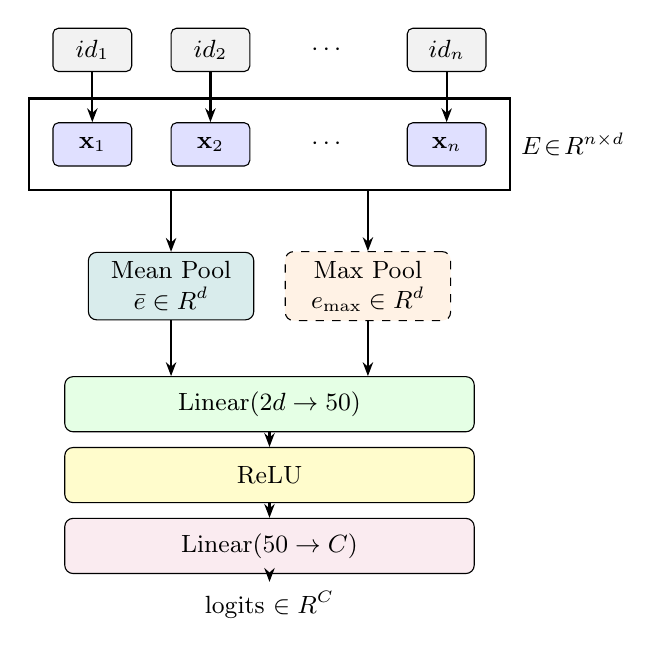
\begin{tikzpicture}[
    token/.style={draw, rounded corners=2pt, minimum width=1.0cm, minimum height=0.55cm,
                  align=center, font=\small\ttfamily, fill=gray!10},
    emb/.style={draw, rounded corners=2pt, minimum width=1.0cm, minimum height=0.55cm,
                align=center, fill=blue!12, font=\small},
    pool/.style={draw, rounded corners=3pt, minimum width=2.1cm, minimum height=0.7cm,
                 align=center, fill=teal!15, font=\small},
    newpool/.style={draw, dashed, rounded corners=3pt, minimum width=2.1cm, minimum height=0.7cm,
                    align=center, fill=orange!10, font=\small},
    fc/.style={draw, rounded corners=3pt, minimum width=5.2cm, minimum height=0.7cm,
               align=center, fill=green!10, font=\small},
    relu/.style={draw, rounded corners=3pt, minimum width=5.2cm, minimum height=0.7cm,
                 align=center, fill=yellow!20, font=\small},
    arr/.style={-{Stealth[length=5pt]}, thick},
]

% Row 1: token IDs
\node[token] (id1) at (0.0, 0)   {$id_1$};
\node[token] (id2) at (1.5, 0)   {$id_2$};
\node        at (3.0, 0)          {\small$\cdots$};
\node[token] (idn) at (4.5, 0)   {$id_n$};

% Row 2: embedding vectors
\node[emb] (x1) at (0.0, -1.2)  {$\mathbf{x}_1$};
\node[emb] (x2) at (1.5, -1.2)  {$\mathbf{x}_2$};
\node       at (3.0, -1.2)        {\small$\cdots$};
\node[emb] (xn) at (4.5, -1.2)  {$\mathbf{x}_n$};

\draw[arr] (id1) -- (x1);
\draw[arr] (id2) -- (x2);
\draw[arr] (idn) -- (xn);

% Box spanning the full embedding sequence
\node[draw, thick, inner sep=0.3cm,
      fit=(x1)(x2)(xn),
      label=right:{\small$E\!\in\!\mathbb{R}^{n\times d}$}] (ebox) {};

% Row 3: arrows drop straight down from ebox at mean/maxp x-positions
\node[pool]    (mean) at (1.0, -3.0) {Mean Pool\\$\bar{e}\in\mathbb{R}^d$};
\node[newpool] (maxp) at (3.5, -3.0) {Max Pool\\$e_{\max}\in\mathbb{R}^d$};

\draw[arr] (ebox.south -| mean) -- (mean.north);
\draw[arr] (ebox.south -| maxp) -- (maxp.north);

% Row 4: linear — mean and max enter vertically
\node[fc] (fc1) at (2.25, -4.5) {Linear$(2d \to 50)$};
\draw[arr] (mean.south) -- (mean |- fc1.north);
\draw[arr] (maxp.south) -- (maxp |- fc1.north);

% Row 5: ReLU (separate layer)
\node[relu] (relu) at (2.25, -5.4) {ReLU};
\draw[arr] (fc1) -- (relu);

% Row 6: output linear
\node[fc, fill=purple!8] (out) at (2.25, -6.3) {Linear$(50 \to C)$};
\draw[arr] (relu) -- (out);

\node[font=\small] (log) at (2.25, -7.05) {logits $\in\mathbb{R}^C$};
\draw[arr] (out) -- (log);
\end{tikzpicture}
\caption{Αρχιτεκτονική \texttt{BaselineDNN} με mean+max pooling
($d$: διάσταση embedding, $C$: αριθμός κλάσεων).
Το πλαίσιο $E$ αγκαλιάζει ολόκληρη την ακολουθία.
Ο κόμβος με διακεκομμένο πλαίσιο είναι η προσθήκη του Ερωτήματος~1
--- στο baseline χρησιμοποιείται μόνο το mean pooling.}
\end{figure}

\subsection{1.2 Σύγκριση και Αποτελέσματα}

Το mean pooling αποτυπώνει τον ``γενικό τόνο'' της πρότασης,
αλλά αδυνατεί να διατηρήσει ισχυρά τοπικά σήματα: ένα token με
έντονη ενεργοποίηση σε κάποια διάσταση αραιώνεται από τον μέσο όρο.
Το max pooling εξάγει, ανά διάσταση, τη μέγιστη τιμή μεταξύ όλων
των tokens, διατηρώντας τα ``ακραία'' αυτά σήματα.
Η συνένωση των δύο δίνει στον γραμμικό ταξινομητή και τη γενική
εικόνα και τα κυρίαρχα χαρακτηριστικά ταυτόχρονα.

\begin{figure}[H]
\centering
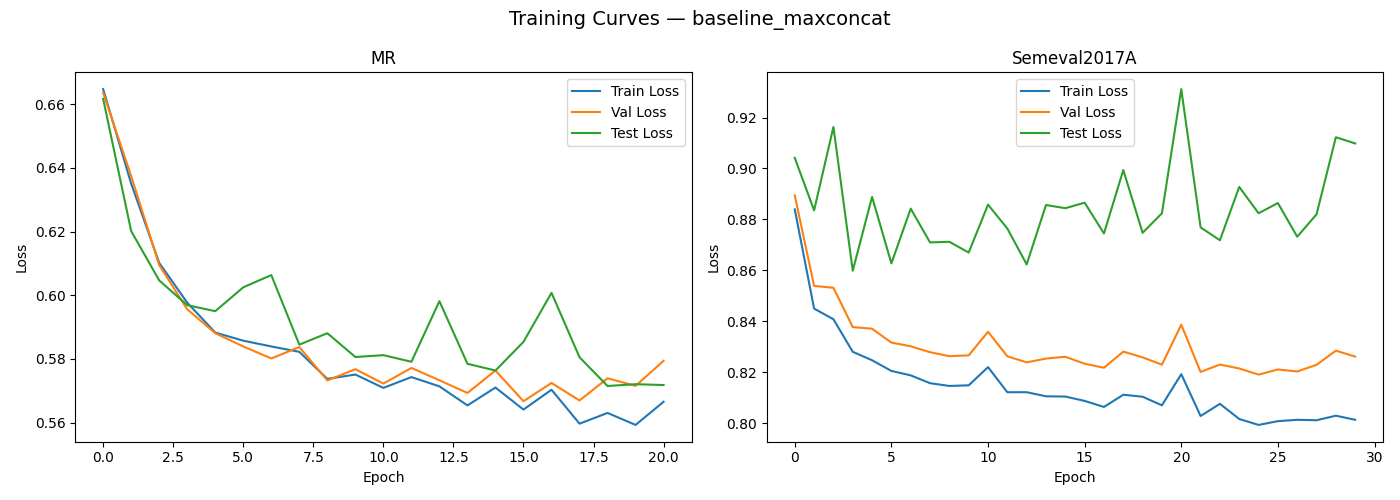
\includegraphics[width=\textwidth]{results/loss_baseline_maxconcat.png}
\caption{Καμπύλες εκπαίδευσης DNN με mean+max pooling στο MR (αριστερά) και Semeval2017A (δεξιά).}
\end{figure}

\lstinputlisting[language={}]{results/baseline_maxconcat_results.txt}

%=======================================================================
\section{Ερώτημα 2: LSTM \& BiLSTM}

\subsection{2.1 Διαχωρισμός Εκπαίδευσης/Επαλήθευσης και Early Stopping}

Σε όλα τα πειράματα (από το baseline μοντέλο και εφεξής) χρησιμοποιούμε
\emph{early stopping} για να αποφύγουμε το overfitting. Η τεχνική απαιτεί
ένα ξεχωριστό \emph{validation set} που κρατάμε εκτός εκπαίδευσης και
παρακολουθούμε την απώλειά του σε κάθε εποχή. Όταν δεν παρατηρείται
βελτίωση για \texttt{PATIENCE} συνεχόμενες εποχές ως προς το καλύτερο
αποτέλεσμα ώς τη στιγμή εκείνη, η εκπαίδευση διακόπτεται και φορτώνεται
αυτό το βέλτιστο checkpoint.

Αξίζει να σημειωθεί ότι δεν μπορούμε να χρησιμοποιήσουμε το
\emph{test set} για τις αποφάσεις early stopping. Αν το κάναμε,
θα εκθέταμε έμμεσα πληροφορία του test set στη διαδικασία επιλογής
μοντέλου, οδηγώντας σε τεχνητά βελτιωμένα αποτελέσματα. Αυτός
είναι ο λόγος που στις καμπύλες εκπαίδευσης παρατηρούμε συνήθως:
\[
    \mathcal{L}_{\text{train}} < \mathcal{L}_{\text{val}} < \mathcal{L}_{\text{test}}
\]
Το μοντέλο ελαχιστοποιεί ενεργά την απώλεια στα training data σε
κάθε βήμα, οπότε το train loss τείνει να είναι χαμηλό. Το validation
set επηρεάζει έμμεσα την εκπαίδευση μέσω των αποφάσεων early stopping,
με αποτέλεσμα το validation loss να είναι υψηλότερο. Το test set δεν
επηρεάζει καθόλου τη διαδικασία, οπότε αντικατοπτρίζει την πραγματική
γενίκευση και αναμένεται να είναι ελαφρώς υψηλότερο ακόμα και από το
validation loss. Καθώς ο ρόλος των training data στη μάθηση του μοντέλου είναι πολύ
πιο θεμελιώδης από την ακριβή εύρεση του βέλτιστου σημείου early
stopping, δεσμεύουμε μόνο το $20\%$ του training set για validation,
ώστε το μεγαλύτερο μέρος να παραμένει διαθέσιμο για εκπαίδευση.

\begin{lstlisting}
# training.py -- torch_train_val_split
train_loader, val_loader = torch_train_val_split(
    train_set, BATCH_SIZE, BATCH_SIZE, val_size=VAL_SIZE
)
stopper = EarlyStopper(model, save_path, patience=PATIENCE)

for epoch in range(1, epochs + 1):
    train_dataset(epoch, train_loader, model, criterion, optimizer)
    val_loss, _ = eval_dataset(val_loader, model, criterion)
    if stopper.early_stop(val_loss):
        break

model.load_state_dict(torch.load(save_path))  # restore best checkpoint
\end{lstlisting}

Η \texttt{EarlyStopper} αποθηκεύει αυτόματα το checkpoint κάθε φορά που
το validation loss βελτιώνεται, ώστε μετά τη διακοπή να φορτωθεί
η βέλτιστη έκδοση και όχι η τελευταία.

\subsection{2.2 LSTM}

Το LSTM, σε αντίθεση με τον μέσο όρο embeddings, επεξεργάζεται τις
λέξεις \emph{σειριακά} διατηρώντας δύο εσωτερικές καταστάσεις: το
\emph{hidden state} $h_i$, που αποτελεί την έξοδο κάθε βήματος και
λειτουργεί ως βραχυπρόθεσμη μνήμη, και το \emph{cell state} $c_i$,
που διαδίδεται από unit σε unit μέσα στην αλυσίδα του LSTM ως
μακροπρόθεσμη μνήμη, χωρίς να εκτίθεται ως έξοδος στα layers
πάνω από αυτό. Κάθε βήμα
παράγει ένα $h_i$ που λαμβάνει υπόψη τόσο την τρέχουσα λέξη
$\mathbf{x}_i$ όσο και τα συμφραζόμενα.

Ο μηχανισμός θυρών (forget, input, output gates) ρυθμίζει ποια
πληροφορία διατηρείται ή απορρίπτεται, επιτρέποντας στο δίκτυο
να μαθαίνει μακρινές εξαρτήσεις χωρίς το vanishing gradient των
απλών RNNs. Χρησιμοποιούμε ως αναπαράσταση κειμένου την τελευταία
\emph{πραγματική} έξοδο $h_N$, όπου $N$ είναι το πραγματικό μήκος
της πρότασης (όχι το padded μήκος). Τα πραγματικά μήκη υπολογίστηκαν
στο Ζητούμενο~3 της προπαρασκευής και χρησιμοποιούνται εδώ για να
επιλέξουμε το σωστό timestep:

\begin{lstlisting}
# models.py -- LSTM.forward
X = torch.nn.utils.rnn.pack_padded_sequence(
    embeddings, lengths.cpu(), batch_first=True, enforce_sorted=False
)
ht, _ = self.lstm(X)
ht, _ = torch.nn.utils.rnn.pad_packed_sequence(ht, batch_first=True)

# pick the actual last token, not the padded end
representations = ht[torch.arange(batch_size), lengths - 1]
logits = self.linear(representations)
return logits
\end{lstlisting}

\begin{figure}[H]
\centering
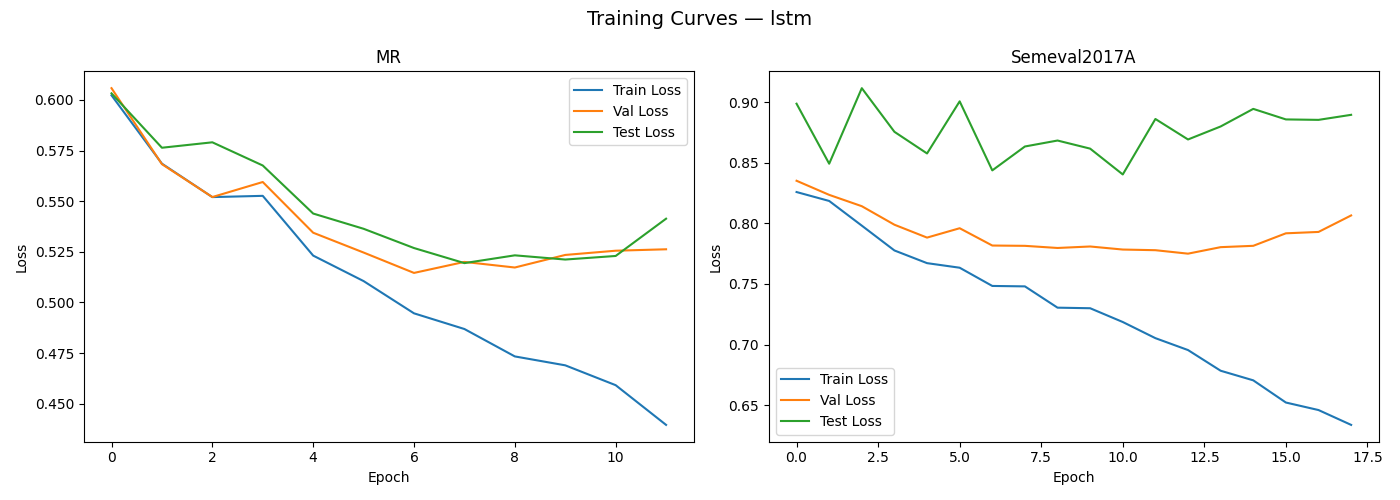
\includegraphics[width=\textwidth]{results/loss_lstm.png}
\caption{Καμπύλες εκπαίδευσης LSTM στο MR (αριστερά) και Semeval2017A (δεξιά).}
\end{figure}

\lstinputlisting[language={}]{results/lstm_results.txt}

\subsection{2.3 Αμφίδρομο LSTM (BiLSTM)}

Το BiLSTM εκτελεί δύο LSTM παράλληλα: ένα από αριστερά προς τα
δεξιά και ένα από δεξιά προς τα αριστερά. Η αναπαράσταση κάθε
θέσης $i$ είναι η συνένωση των δύο hidden states:
\[
    h_i = [\,\overrightarrow{h}_i \;\|\; \overleftarrow{h}_i\,],
    \quad h_i \in \mathbb{R}^{2H}
\]

Αυτό επιτρέπει σε κάθε λέξη να ``γνωρίζει'' τόσο το αριστερό
(τι προηγήθηκε) όσο και το δεξί (τι ακολουθεί) πλαίσιο, κάτι
κρίσιμο στη φυσική γλώσσα όπου η σημασία εξαρτάται συχνά και
από τις μεταγενέστερες λέξεις.

Χρειάζεται λοιπόν να διπλασιάσουμε το μέγεθος της αναπαράστασης
που περνάει από τον τελικό γραμμικό μετασχηματισμό. Το υπόλοιπο
μέρος της υλοποίησης γίνεται από την PyTorch θέτοντας την παράμετρο
\texttt{bidirectional} κατά την κατασκευή του LSTM module.

\begin{lstlisting}
# models.py -- LSTM.__init__
self.representation_size = (
    2 * self.hidden_size if self.bidirectional else self.hidden_size
)
\end{lstlisting}

\begin{figure}[H]
\centering
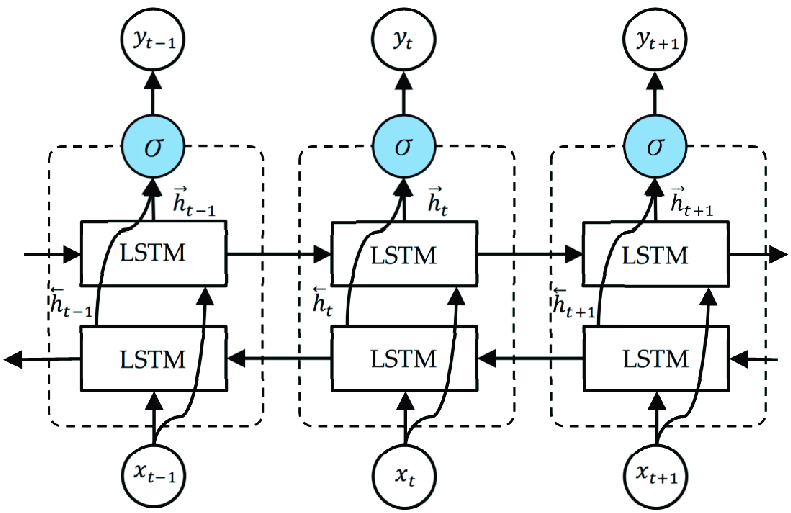
\includegraphics[width=\textwidth]{biLSTMarch.png}
\caption{Αρχιτεκτονική BiLSTM. Η έξοδος $y_N$ στο τελευταίο
πραγματικό token της ακολουθίας περνά από ένα γραμμικό layer
$\mathbb{R}^{2H} \to \mathbb{R}^C$ για την τελική ταξινόμηση.}
\end{figure}

\begin{figure}[H]
\centering
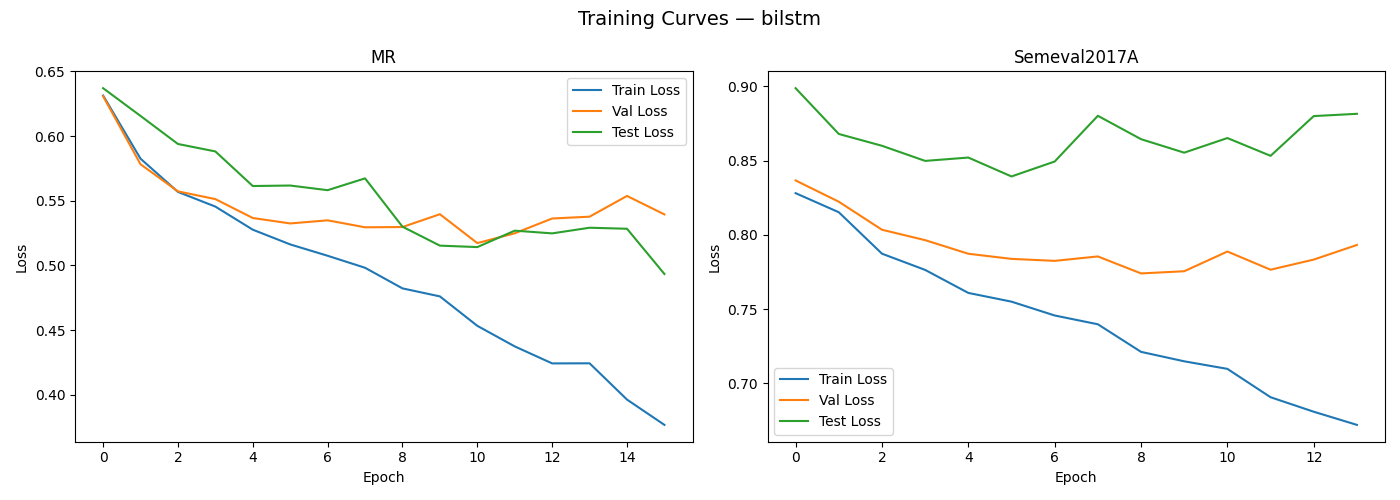
\includegraphics[width=\textwidth]{results/loss_bilstm.png}
\caption{Καμπύλες εκπαίδευσης BiLSTM στο MR (αριστερά) και Semeval2017A (δεξιά).}
\end{figure}

\lstinputlisting[language={}]{results/bilstm_results.txt}

Το BiLSTM βελτιώνει σταθερά την επίδοση σε σχέση με το
μονοκατευθυντικό LSTM, ιδιαίτερα στο MR ($+0.7$\% F1). Η βελτίωση
επιβεβαιώνει ότι η πληροφορία από τα δεξιά συμφραζόμενα είναι
χρήσιμη για την ανάλυση συναισθήματος.

%=======================================================================
\section{Ερώτημα 3: Self-Attention}

\subsection{3.1 Υλοποίηση και Αποτελέσματα}

Ο μηχανισμός self-attention αντικαθιστά τη σειριακή επεξεργασία του LSTM
με μια \emph{παράλληλη} λειτουργία: κάθε λέξη ``επικοινωνεί'' ταυτόχρονα με
όλες τις υπόλοιπες στην πρόταση, ώστε το αρχικό της embedding να αντικατασταθεί
από μια σημασιολογικά εμπλουτισμένη αναπαράσταση βασισμένη στα συμφραζόμενα.

\medskip
Την λειτουργία αυτή εκτελεί η κλάση \texttt{Head}, με τον τρόπο που απεικονίζεται παρακάτω:

\begin{figure}[H]
\centering
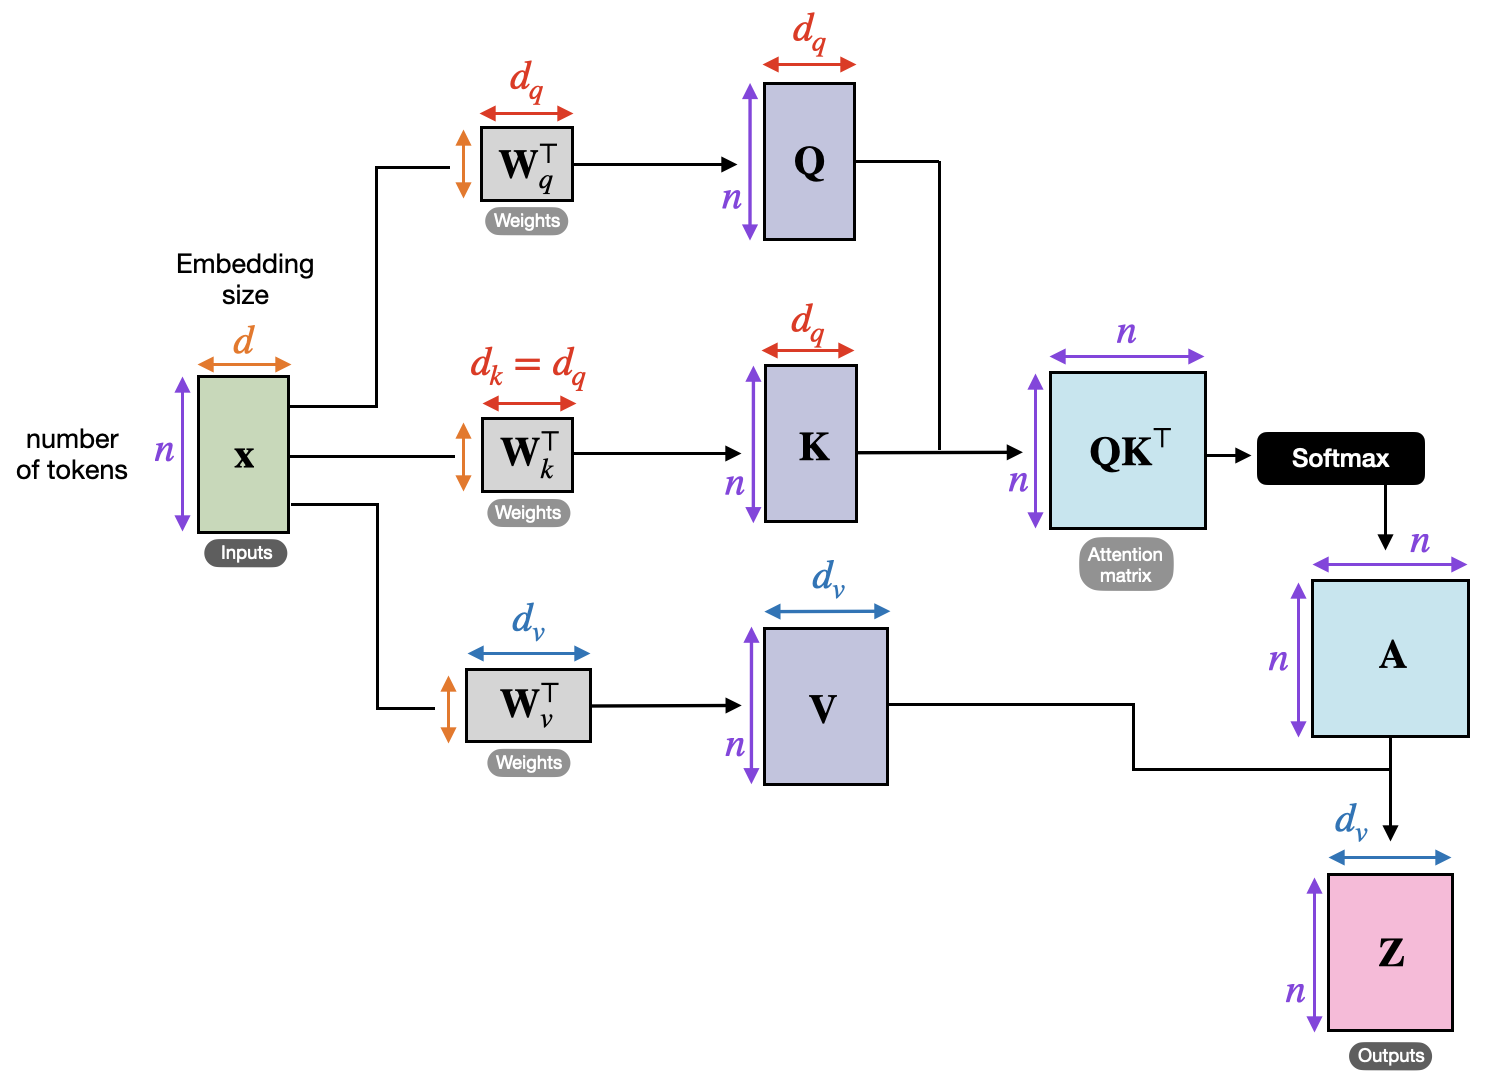
\includegraphics[width=0.82\textwidth]{selfAttention.png}
\caption{Διάγραμμα single-head self-attention.
Η είσοδος $X \in \mathbb{R}^{d \times n}$ είναι ο πίνακας αναπαραστάσεων
όλων των tokens (embedding matrix).
Τρεις γραμμικοί μετασχηματισμοί $W^Q, W^K, W^V$ παράγουν τους πίνακες
$Q, K, V \in \mathbb{R}^{d_k \times n}$.
Τα τελικά βάρη attention $A \in \mathbb{R}^{n \times n}$ προκύπτουν ως $\text{softmax}(QK^T/\sqrt{d_k})$.
Η έξοδος $Z = AV \in \mathbb{R}^{d_v \times n}$ είναι η νέα, εμπλουτισμένη, αναπαράσταση
κάθε token.}
\end{figure}

Η είσοδος $X$ της \texttt{Head} κατασκευάζεται στο \texttt{forward}
του \texttt{SimpleSelfAttentionModel} ως άθροισμα token embedding
και position embedding κάθε θέσης:

\begin{lstlisting}
# attention.py -- SimpleSelfAttentionModel.forward
tok_emb = self.token_embedding_table(x)          # (B, T, d)
pos_emb = self.position_embedding_table(
    torch.arange(T, device=x.device))             # (T, d)
x = tok_emb + pos_emb                            # X: (B, T, d)
x = x + self.sa(self.ln1(x))                     # weighted aggregation + residual
x = x + self.ffwd(self.ln2(x))                   # separate feed-forward block + residual
\end{lstlisting}

\medskip
Ακολουθεί ένα feed-forward layer, και στη συνέχεια εφαρμόζεται
masked average-pooling για να εξαχθεί αναπαράσταση ολόκληρης
της πρότασης. Το τελικό γραμμικό classification layer ακολουθεί
την ίδια λογική με τα προηγούμενα ερωτήματα.

\begin{figure}[H]
\centering
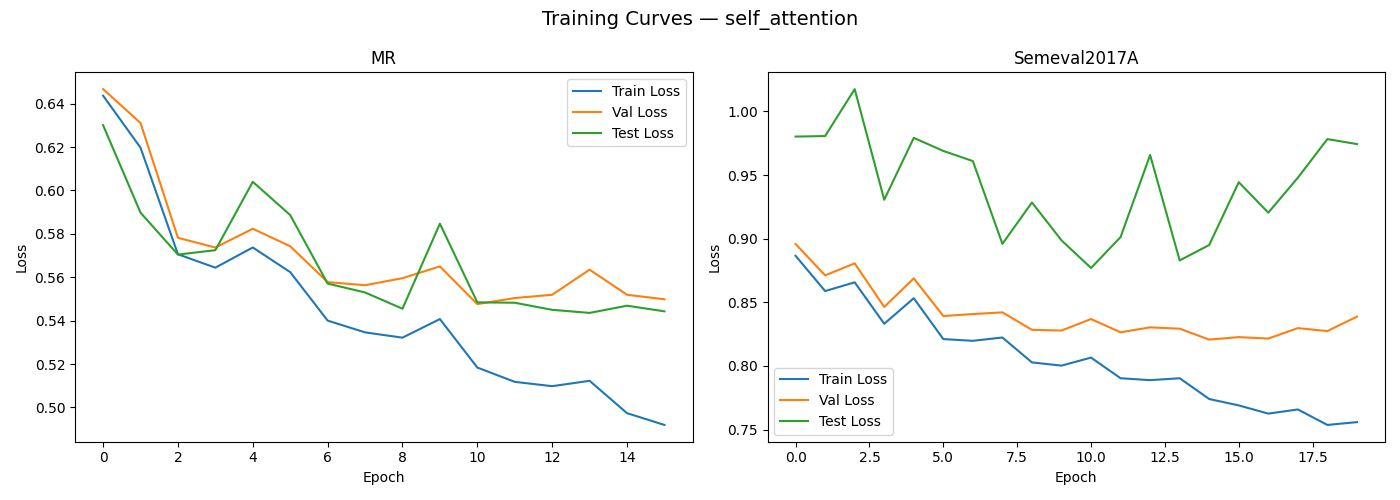
\includegraphics[width=\textwidth]{results/loss_self_attention.png}
\caption{Καμπύλες εκπαίδευσης Self-Attention στο MR (αριστερά) και Semeval2017A (δεξιά).}
\end{figure}

\lstinputlisting[language={}]{results/self_attention_results.txt}

Το single-head self-attention επιτυγχάνει 69.6\% F1 στο MR και
57.6\% στο Semeval2017A. Η επίδοση υπολείπεται του LSTM (71.8\% / 59.4\%)
και του BiLSTM, κάτι αναμενόμενο για single-head χωρίς πολλαπλή
εξειδίκευση των heads. Αξίζει να σημειωθεί ότι το LSTM και BiLSTM
αποδίδουν ιδιαίτερα καλά εδώ λόγω του σχετικά μικρού μήκους
των προτάσεων στα datasets: η σειριακή επεξεργασία δεν υποφέρει
από vanishing gradient σε τόσο σύντομες ακολουθίες, οπότε δεν
αναδεικνύεται η αδυναμία της.

\subsection{3.2 Queries, Keys, Values και Position Embeddings}

Στην κλάση \texttt{Head} (\texttt{attention.py}), κάθε token παράγει
τρία διανύσματα μέσω των εκπαιδεύσιμων γραμμικών προβολών $W^Q, W^K, W^V$, αντίστοιχα:

\begin{itemize}
    \item \textbf{Query} ($q$, ``τι πληροφορία ψάχνω;''): αντιπροσωπεύει
    αυτό που θέλει να μάθει το token από τα υπόλοιπα.
    \item \textbf{Key} ($k$, ``τι πληροφορία προσφέρω;''): αντιπροσωπεύει
    αυτό που ``διαφημίζει'' το token ως περιεχόμενό του.
    \item \textbf{Value} ($v$, ``ποιο είναι το πραγματικό μου περιεχόμενο;''):
    η πληροφορία που μεταφέρεται αν η ``ερώτηση'' ταιριάξει με το ``κλειδί''.
\end{itemize}

\medskip
Όπως φαίνεται στο παραπάνω διάγραμμα, η έξοδος του head υπολογίζεται ως:
\[
    Z = \text{softmax}\!\left(\frac{QK^T}{\sqrt{d_k}}\right) V
\]
Ο παράγοντας $\sqrt{d_k}$ στον παρονομαστή συνίσταται για αριθμητική
σταθερότητα: αν τα στοιχεία των $q$ και $k$ έχουν μέση τιμή 0 και διακύμανση 1,
το εσωτερικό τους γινόμενο έχει διακύμανση $d_k$.
Για μεγάλο $d_k$ τα γινόμενα γίνονται αριθμητικά μεγάλα, ωθώντας το softmax
σε περιοχές κορεσμού με μηδενικές σχεδόν κλίσεις.
Η διαίρεση με $\sqrt{d_k}$ ανάγει τη διακύμανση πίσω στη μονάδα,
αποτρέποντας το πρόβλημα αυτό.

Στην υλοποίησή μας επιλέχθηκε $d_k = d$, δηλαδή οι προβολές $Q, K, V$
έχουν την ίδια διάσταση με τα embeddings.

\medskip
Τα \textbf{position embeddings} (\texttt{position\_embedding\_table}
στο \texttt{SimpleSelfAttentionModel}) είναι ένας εκπαιδεύσιμος πίνακας
μεγέθους $T_{\max} \times d$. Ο μηχανισμός attention από μόνος του
δεν έχει εγγενή έννοια θέσης: λειτουργεί σε ένα \emph{σύνολο}
διανυσμάτων και θα έδινε τα ίδια αποτελέσματα ανεξαρτήτως της
σειράς τους. Προσθέτοντας το position embedding $p_i$ στο token
embedding $e_i$ ($x_i = e_i + p_i$), το μοντέλο αποκτά πρόσβαση
στη θέση κάθε token στην ακολουθία, επιτρέποντάς του να διαφοροποιήσει
π.χ.\ ``not good'' από ``good not''.

%=======================================================================
\section{Ερώτημα 4: MultiHead Attention}

Αντί ενός μόνο attention head, χρησιμοποιούμε $h$ heads
παράλληλα, κάθε ένα με $d_k = d / h$ διαστάσεις.
Κάθε head μαθαίνει διαφορετικές σχέσεις μεταξύ tokens:
ένα μπορεί να εστιάζει σε σχέσεις ``γειτονικών'' λέξεων,
ένα άλλο σε μακρινές εξαρτήσεις, ένα τρίτο σε σημασιολογική
ομοιότητα κλπ. Οι έξοδοι συνενώνονται και προβάλλονται
πίσω στην αρχική διάσταση:
\[
    \text{MHA}(x) = [h_1 \,\|\, h_2 \,\|\, \cdots \,\|\, h_h] \, W^O
\]

\begin{figure}[H]
\centering
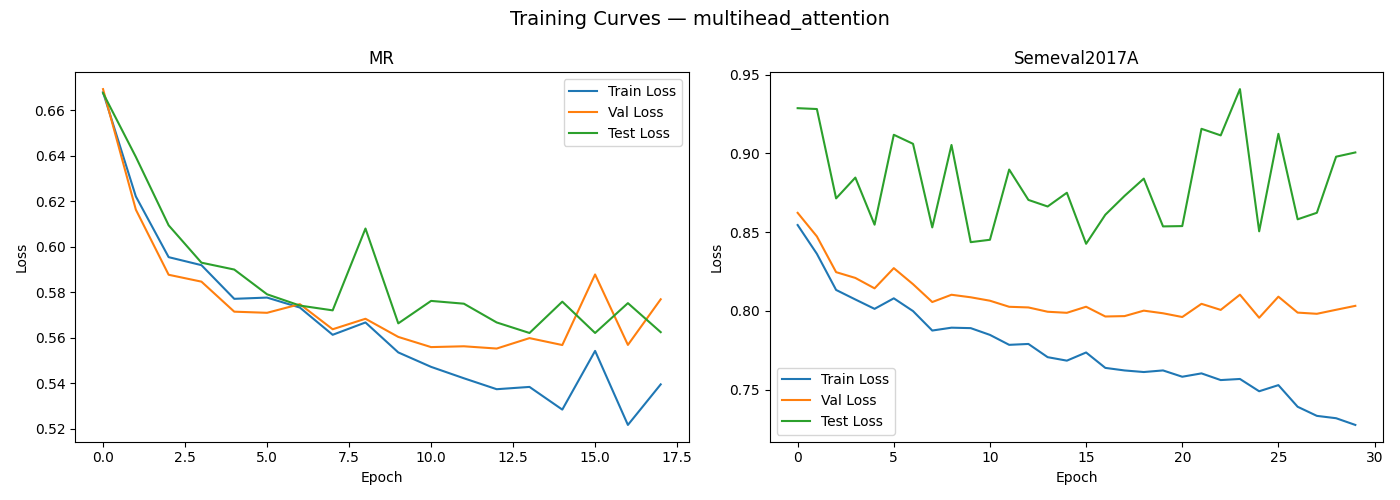
\includegraphics[width=\textwidth]{results/loss_multihead_attention.png}
\caption{Καμπύλες εκπαίδευσης MultiHead Attention στο MR (αριστερά) και Semeval2017A (δεξιά).}
\end{figure}

\lstinputlisting[language={}]{results/multihead_attention_results.txt}

Η χρήση πολλαπλών heads βελτιώνει την επίδοση σε σχέση
με το single-head self-attention ($+2$\% F1 στο MR),
καθώς κάθε head εξειδικεύεται σε διαφορετικό τύπο σχέσης.

%=======================================================================
\section{Ερώτημα 5: Transformer Encoder}

\subsection{Αρχιτεκτονική}

Ο Transformer Encoder αποτελείται από πολλαπλά \texttt{Block},
κάθε ένα με:
\begin{enumerate}
    \item MultiHead Self-Attention + residual connection + Layer Normalization
    \item Feed-Forward Network ($d \to 4d \to d$) + residual connection + Layer Normalization
\end{enumerate}

Η βασική διαφορά από το MultiHeadAttentionModel είναι:
\begin{itemize}
    \item \textbf{Στοίβαξη} πολλαπλών blocks ($N$ layers), που
    επιτρέπει σταδιακή εξαγωγή υψηλότερου επιπέδου αναπαραστάσεων.
    \item \textbf{Residual connections} ($x + f(x)$), που
    εξασφαλίζουν ομαλή ροή gradient και επιτρέπουν βαθύτερα δίκτυα.
    \item \textbf{Layer Normalization}, που σταθεροποιεί την εκπαίδευση.
\end{itemize}

\subsection{Υπερπαράμετροι}

Στην κλασική αρχιτεκτονική ``Attention Is All You Need'', οι default τιμές
είναι: $d_{\text{model}} = 512$, $h = 8$ heads, $N = 6$ layers,
$d_{ff} = 2048$.

Στην υλοποίησή μας χρησιμοποιήσαμε Twitter GloVe embeddings
($d = 200$), $h = 5$ heads, $N = 5$ layers, $d_{ff} = 800$,
λόγω του μικρότερου μεγέθους embeddings και dataset.

\subsection{Αποτελέσματα}

\begin{figure}[H]
\centering
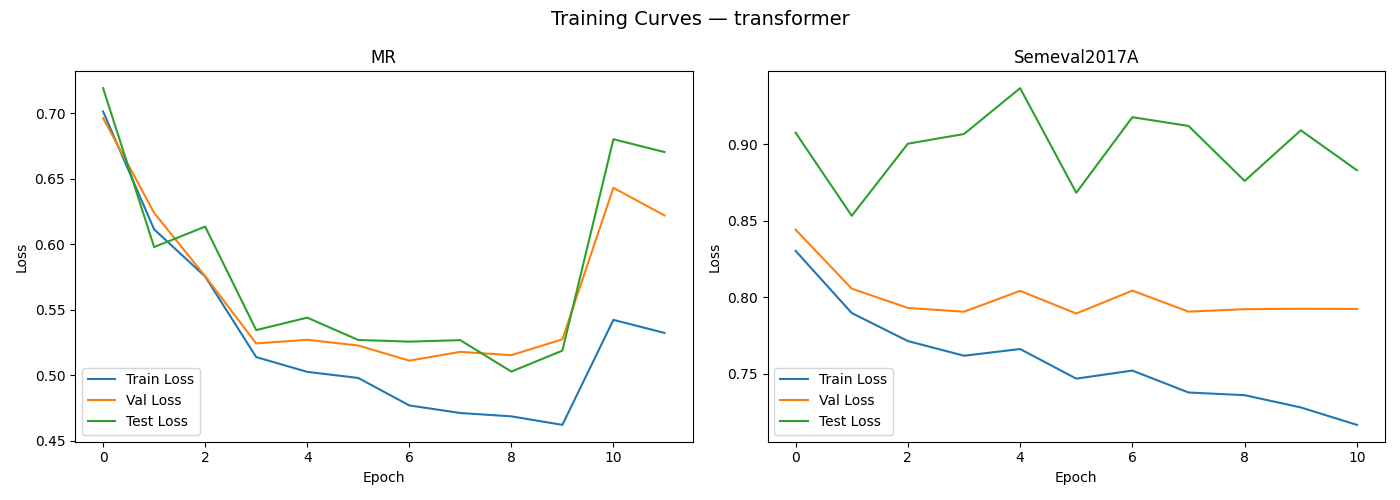
\includegraphics[width=\textwidth]{results/loss_transformer.png}
\caption{Καμπύλες εκπαίδευσης Transformer Encoder στο MR (αριστερά) και Semeval2017A (δεξιά).}
\end{figure}

\lstinputlisting[language={}, firstline=143, lastline=153]{results/transformer_results.txt}

Ο Transformer Encoder πετυχαίνει την υψηλότερη επίδοση μεταξύ
των μοντέλων Ερωτημάτων 1--5 (73.1\% F1 στο MR, 60.3\% στο
Semeval2017A), αποδεικνύοντας ότι η βαθύτερη αρχιτεκτονική
αξιοποιεί καλύτερα τις σχέσεις μεταξύ tokens.

%=======================================================================
\section{Ερώτημα 6: Pre-Trained Transformers (Zero-Shot)}

Αξιολογήσαμε 3 προ-εκπαιδευμένα μοντέλα ανά dataset σε zero-shot
κατηγοριοποίηση (χωρίς εκπαίδευση, μόνο inference).

\subsection{MR Dataset}

\begin{center}
\begin{tabular}{lccc}
\toprule
Μοντέλο & Accuracy & Recall & F1 \\
\midrule
DistilBERT-SST2 & 0.891 & 0.891 & 0.891 \\
RoBERTa-large (siebert) & \textbf{0.924} & \textbf{0.924} & \textbf{0.924} \\
BERT-SST2 (textattack) & 0.899 & 0.899 & 0.899 \\
\bottomrule
\end{tabular}
\end{center}

\subsection{Semeval2017A Dataset}

\begin{center}
\begin{tabular}{lccc}
\toprule
Μοντέλο & Accuracy & Recall & F1 \\
\midrule
twitter-roberta-base & \textbf{0.724} & 0.723 & \textbf{0.722} \\
bertweet-base & 0.718 & \textbf{0.730} & 0.718 \\
sentiment-roberta-large-3c & 0.698 & 0.649 & 0.669 \\
\bottomrule
\end{tabular}
\end{center}

\subsection{Σχολιασμός}

Τα pre-trained μοντέλα υπερτερούν κατά πολύ ($+15$--$20$\% F1)
σε σχέση με τα μοντέλα που εκπαιδεύσαμε (Q1--Q5). Αυτό αποδίδεται
στο ότι τα μοντέλα αυτά:
\begin{itemize}
    \item Χρησιμοποιούν contextualized embeddings αντί static.
    \item Είναι εκπαιδευμένα σε τεράστια corpora (εκατοντάδες GB κειμένου).
    \item Έχουν ήδη κάνει fine-tuning σε sentiment analysis tasks.
\end{itemize}

Στο Semeval2017A, τα μοντέλα εκπαιδευμένα σε Twitter
(roberta-base-sentiment, bertweet) υπερτερούν αισθητά
σε σχέση με ένα general-purpose μοντέλο, επιβεβαιώνοντας ότι
η αντιστοιχία domain μεταξύ pre-training και εφαρμογής είναι κρίσιμη.

%=======================================================================
\section{Ερώτημα 7: Fine-Tuning Pre-Trained Transformers}

Κάνουμε fine-tuning βασικών (base) μοντέλων στα δικά μας
datasets (5 epochs, batch size 32, lr $= 5 \times 10^{-5}$).

\subsection{MR Dataset}

\begin{center}
\begin{tabular}{lcccc}
\toprule
Μοντέλο & Epochs & Accuracy & Recall & F1 \\
\midrule
bert-base-uncased & 5 & 0.849 & 0.840 & 0.848 \\
distilbert-base-uncased & 5 & 0.840 & 0.843 & 0.840 \\
roberta-base & 5 & \textbf{0.881} & 0.837 & \textbf{0.875} \\
\bottomrule
\end{tabular}
\end{center}

\subsection{Semeval2017A Dataset}

\begin{center}
\begin{tabular}{lcccc}
\toprule
Μοντέλο & Epochs & Accuracy & Recall & F1 \\
\midrule
twitter-roberta-base & 5 & \textbf{0.703} & \textbf{0.718} & \textbf{0.704} \\
bertweet-base (vinai) & 5 & 0.700 & 0.717 & 0.702 \\
bert-base-cased & 5 & 0.674 & 0.673 & 0.669 \\
\bottomrule
\end{tabular}
\end{center}

\subsection{Σχολιασμός}

Τα fine-tuned μοντέλα βελτιώνουν σημαντικά τα μοντέλα Q1--Q5
αλλά υστερούν σε σχέση με τα ήδη fine-tuned μοντέλα του Q6,
καθώς αυτά εκπαιδεύτηκαν σε μεγαλύτερα και πιο αντιπροσωπευτικά
sentiment datasets.

Στο Semeval, τα domain-matched μοντέλα (Twitter) ξεπερνούν
το γενικό bert-base-cased κατά $\sim$3\% F1, επιβεβαιώνοντας
ξανά τη σημασία του domain-specific pre-training.

Αξιοσημείωτο είναι ότι ακόμη και 5 epochs fine-tuning
μπορούν να φέρουν ένα base model κοντά στην επίδοση ενός
ειδικού sentiment model --- η δύναμη του transfer learning
σε δράση.

%=======================================================================
\section{Ερώτημα 8: Ανάλυση Κώδικα GPT με ChatGPT}

Χρησιμοποιήσαμε το ChatGPT για ανάλυση, αξιολόγηση και
refactoring του κώδικα ``Let's build GPT'' του A.\ Karpathy.

\subsection*{Επεξήγηση κώδικα}

Το ChatGPT περιέγραψε λεπτομερώς κάθε τμήμα: τη δημιουργία
του vocabulary (character-level tokenization), τη δομή του
\texttt{Head} (scaled dot-product attention), τον τρόπο που
η causal mask εμποδίζει κάθε θέση να ``κοιτάξει'' μελλοντικά
tokens, και τη λειτουργία του \texttt{Block} ως μονάδα
``επικοινωνίας + επεξεργασίας''.

\subsection*{Αξιολόγηση}

Ως θετικά αναγνώρισε τη modular δομή (Head, Block, GPT), τη χρήση
residual connections για σταθερότητα gradient, και το pre-norm
(LayerNorm πριν, όχι μετά, κάθε sublayer). Ως μειονεκτήματα
επισήμανε: (α) την απουσία weight tying (embedding \& output layer),
(β) τη μη χρήση \texttt{nn.MultiheadAttention} του PyTorch,
(γ) τη σταθερή χρήση dropout χωρίς δυνατότητα αποσύνδεσης
κατά την αξιολόγηση μέσω \texttt{model.eval()}.

\subsection*{Refactoring}

Πρότεινε τη συγχώνευση των Q/K/V projections σε ένα μόνο
\texttt{nn.Linear(n\_embd, 3*n\_embd)} για αποδοτικότερο
υπολογισμό, και τη μετατροπή σε \texttt{nn.MultiheadAttention}
για αξιοποίηση βελτιστοποιημένων CUDA kernels.

\subsection*{Σχόλια}

Το ChatGPT ήταν πολύ αποτελεσματικό στην εξήγηση αρχιτεκτονικών
αποφάσεων και στον εντοπισμό καλών πρακτικών. Ωστόσο, ορισμένες
προτάσεις refactoring (π.χ.\ weight tying) θα μπορούσαν να
αλλάξουν τη συμπεριφορά εκπαίδευσης --- σημαντικό να ελέγχονται
πάντα πειραματικά.

%=======================================================================
\section{Συγκριτικός Πίνακας Αποτελεσμάτων}

\begin{center}
\small
\begin{tabular}{l|ccc|ccc}
\toprule
 & \multicolumn{3}{c|}{\textbf{MR}} & \multicolumn{3}{c}{\textbf{Semeval2017A}} \\
\textbf{Μοντέλο} & Acc & Rec & F1 & Acc & Rec & F1 \\
\midrule
Baseline (mean) & .704 & .704 & .704 & .563 & .558 & .532 \\
Baseline (mean+max) & .666 & .667 & .666 & .600 & .594 & .575 \\
LSTM & .719 & .721 & .718 & .608 & .599 & .594 \\
BiLSTM & .727 & .733 & .725 & .618 & .628 & .587 \\
Self-Attention & .696 & .696 & .696 & .612 & .624 & .576 \\
MultiHead Attention & .716 & .717 & .716 & .620 & .620 & .589 \\
Transformer Encoder & .731 & .731 & .731 & .622 & .610 & .603 \\
\midrule
Pre-trained (best) & .924 & .924 & .924 & .724 & .723 & .722 \\
Fine-tuned (best) & .881 & .837 & .875 & .703 & .718 & .704 \\
\midrule
ChatGPT (zero-shot) & 1.00 & 1.00 & 1.00 & 1.00 & 1.00 & 1.00 \\
\bottomrule
\end{tabular}
\end{center}

Παρατηρήσεις:
\begin{itemize}
    \item Τα sequence-aware μοντέλα (LSTM, BiLSTM, Transformer)
    υπερτερούν σταθερά του bag-of-words baseline, καθώς
    αξιοποιούν τη σειρά και τα συμφραζόμενα.
    \item Ο Transformer Encoder πετυχαίνει την υψηλότερη
    επίδοση μεταξύ Q1--Q5, χάρη στη βαθύτερη αρχιτεκτονική
    και τα residual connections.
    \item Τα pre-trained μοντέλα κυριαρχούν, αποδεικνύοντας
    τη δύναμη του transfer learning και των contextualized
    embeddings.
    \item Το ChatGPT πετυχαίνει τέλεια ακρίβεια στο δοκιμαστικό
    δείγμα, αλλά η σύγκριση δεν είναι δίκαιη: αξιολογήθηκε
    σε μικρό υποσύνολο (40--60 δείγματα) ενώ τα υπόλοιπα
    μοντέλα αξιολογήθηκαν στο πλήρες test set.
\end{itemize}

%=======================================================================
\section{Bonus: LoRA Fine-Tuning}

Συγκρίναμε πλήρες fine-tuning και LoRA fine-tuning
του \texttt{textattack/bert-base-uncased-SST-2} στο MR dataset.

\begin{center}
\begin{tabular}{lccccc}
\toprule
Μέθοδος & Trainable \% & Accuracy & Recall & F1 & Loss \\
\midrule
Full fine-tuning & 100\% & 0.900 & 0.876 & 0.898 & 0.597 \\
LoRA ($r = 8$) & 1.2\% & \textbf{0.905} & 0.876 & \textbf{0.902} & \textbf{0.413} \\
\bottomrule
\end{tabular}
\end{center}

\textbf{Σχεδιαστικές επιλογές LoRA:}
\begin{itemize}
    \item Rank $r = 8$ σε όλα τα attention και FFN layers
    (query, key, value, attention output, intermediate, output dense).
    \item Ο classifier head παραμένει πλήρως εκπαιδεύσιμος
    (\texttt{modules\_to\_save}), καθώς είναι μικρός αλλά
    κρίσιμος για το task.
    \item Learning rate $2 \times 10^{-4}$, $\sim$$10\times$
    μεγαλύτερο από full fine-tuning, διότι οι LoRA adapters
    ξεκινούν από μηδενικά βάρη.
\end{itemize}

Το LoRA πετυχαίνει ελαφρώς καλύτερη επίδοση με μόλις 1.2\%
εκπαιδεύσιμες παραμέτρους --- τυπικό αποτέλεσμα, καθώς ο
περιορισμός χαμηλού rank δρα ως regularizer, αποτρέποντας
το overfitting που παρατηρείται στο full fine-tuning μετά
τα 3--4 epochs.

\end{document}
